\documentclass[11pt,letterpaper]{article}
\usepackage[margin=1.0in]{geometry}
\usepackage{amssymb,amsmath,enumerate,mathtools}
\usepackage{graphics,graphicx}
\usepackage{framed, listings}

\lstset{
    language=Verilog,                            % sets the language for the code
    basicstyle=\scriptsize\ttfamily,       % for the actual code
    morekeywords={assign, logic, module, endmodule},  % adds keywords
    deletekeywords={if, do, for},               % removes keywords
    keywordstyle=\bfseries\textbf,                % for keywords
    commentstyle=\scriptsize\ttfamily\emph,     % for comments 
    showstringspaces=false                 % prevents underscores from appearing in output
}

\begin{document}
\begin{flushright}
Andrew Scott\\
E155\\
Lab 3\\
September 28, 2015
\end{flushright}

\begin{center}
Lab 3: Keypad Scanner
\end{center}

\noindent\textbf{Introduction}

In this lab, I added a keypad to the breadboard circuit I had before. I then wrote Verilog code to scan the keyboard and see if any keys were pressed and then display the last two pressed keys on the seven segment display.

\noindent\textbf{Design and Testing Methodology}

The difficulty in this lab was mostly in the Verilog code, so there were little design choices to make for the hardware/breadboard. I added a reset switch to attach to the reset signal in my hardware (I didn't have a breadboard switch before). Also, I connected the column pins from my keypad to pull down resistors so that the utility board pins would see valid logic levels when the voltage on the keypad pins were low. I tested the keypad with a multimeter to check that the pins were becoming connected when a key was pressed, and then I tested the whole circuit by making sure everything worked after loading my Verilog code onto the FPGA.

The software side of this lab required many design decisions that were not easy. I decided to check which keys were pressed down by polling the rows one at a time and then checking the output from the columns to see if any of them were high. To accomplish this, I used a finite state machine whose states were the row currently being polled. The state machine then switched to the new state when a counter register filled up. I made the counter 13 bits long, which makes the row poller switch to a new row every 0.0002 seconds, which was plenty fast to catch any key presses. I then had to decide how to handle the key bounce problem. The solution I came up with was another finite state machine. This FSM has four states - no press, current press, recent press and ending press. The first two states are self explanatory. The recent press state is reached from the current press state when there's no key currently pressed, and this transition also resets a counter variable. The FSM then stays in the recently pressed state until the counter variable fills up, and then it goes to the ending press state. The ending press state is used to send a write enable signal to the registers holding the values that are displayed on the seven segment display, and then transitions back to the no press or currently pressed state depending on if a key is pressed. The counter to check when to leave the recent press state is 21 bits long. This means that if a key is not pressed down for just over 0.05 seconds (which is longer than any key bounce will last for) the next press will register as a new press. This time is short enough that nobody can press a key twice and have it register as only one press. The bounce checking FSM transitions between states every time an 11 bit counter fills up. This is shorter than the counter for the row poller FSM to ensure that multiple changes can happen while a single row is being pressed. Finally, I added a two register synchronizer to make sure that the column signal had time to resolve itself if a keypad button was released on a clock edge.


\noindent\textbf{Results and Discussion}\\
I was able to finish this entire lab, and everything appears to be working as it is supposed to. I am happy that I simulated my hardware before testing on the breadboard because I noticed some timing issues in my circuit that I was able to fix.

\noindent\textbf{Conclusion}\\
I spent about 9 hours on this lab. 


\pagebreak

\noindent\textbf{Breadboard Schematic}\\\\
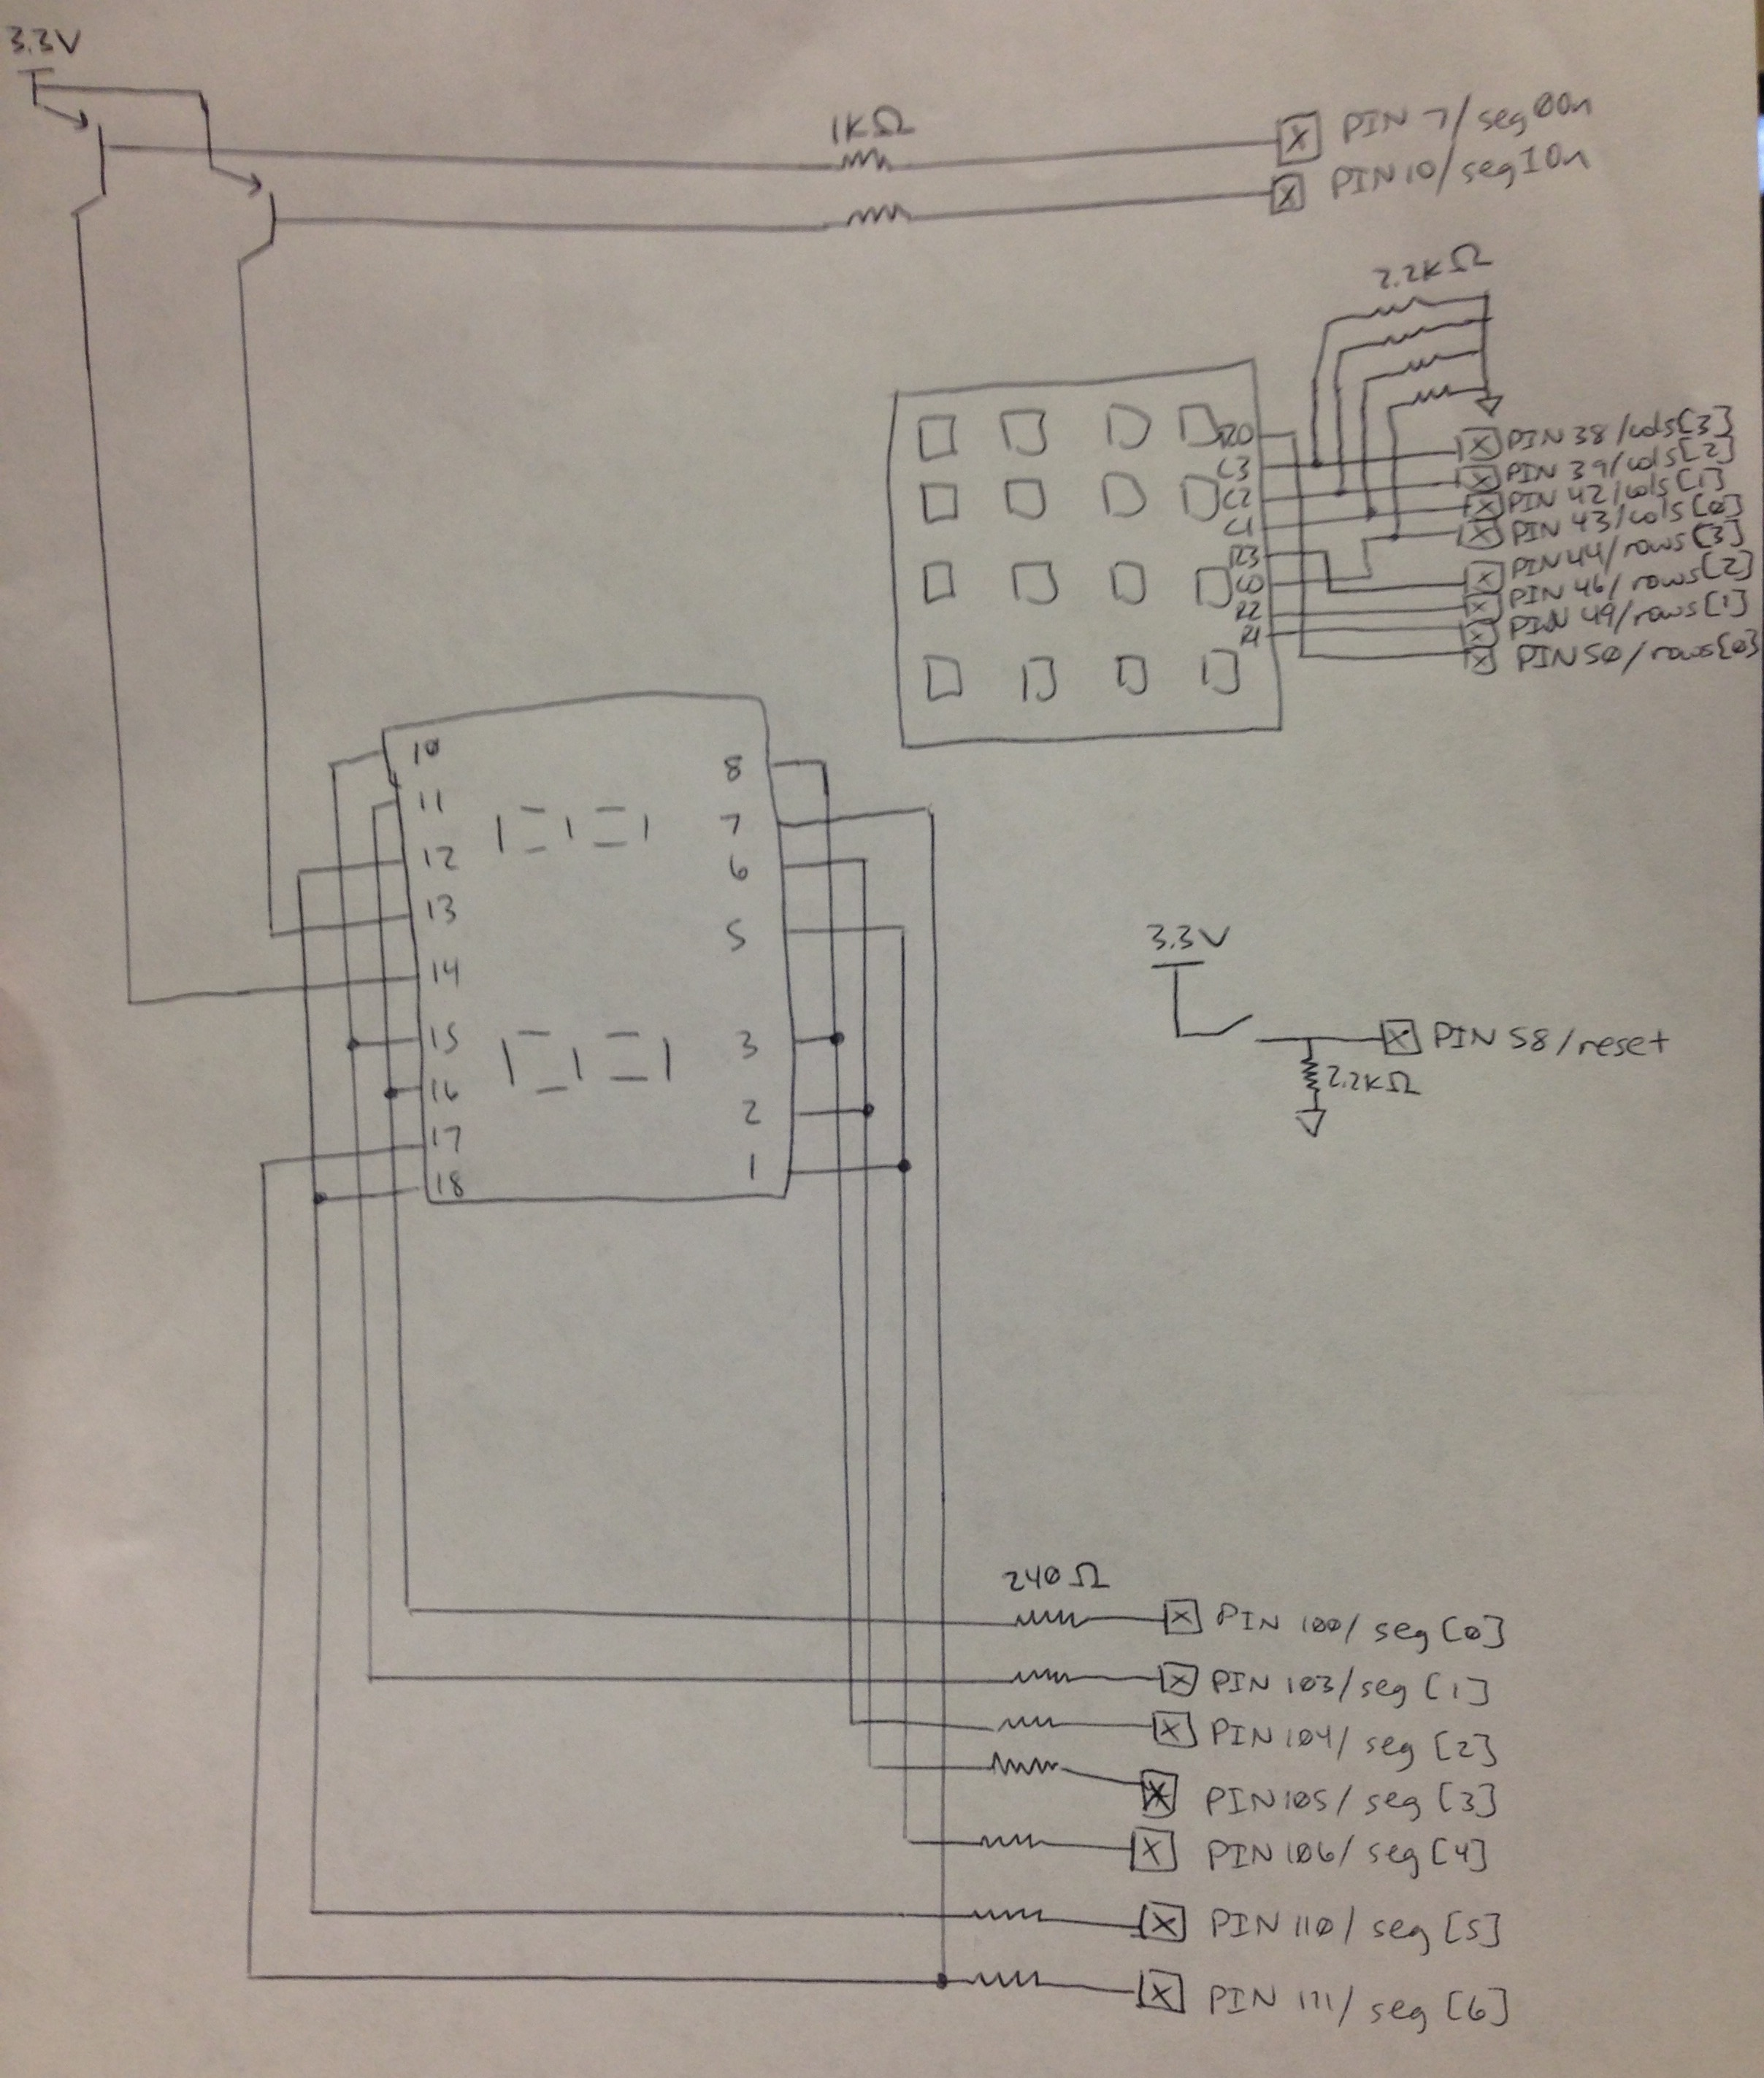
\includegraphics[scale=0.2]{lab3schematic}

\pagebreak

\noindent\textbf{Verilog Code}\\
\lstset{language=Verilog}
\lstinputlisting{lab3_as.sv}

\end{document}

